\documentclass[a4paper,ngerman]{scrartcl}
\renewcommand{\rmdefault}{cmr}
\renewcommand{\sfdefault}{cmss}
\renewcommand{\ttdefault}{cmtt}
\usepackage[T1]{fontenc}
\usepackage[utf8]{inputenc}
\usepackage{array}
\usepackage{refstyle}
\usepackage{float}
\usepackage{enumitem}
\usepackage{amsmath}
%\usepackage{euler}
\usepackage{hyperref}
\makeatletter
\usepackage{multirow}
\usepackage{isotope}
\usepackage{tikz-uml}
\usepackage[section]{placeins}
\flushbottom
\usepackage{geometry}
\geometry{a4paper}
\usepackage[headsepline]{scrpage2}
\usepackage{color}
\usetikzlibrary{circuits.ee.IEC}
%\usepackage{beramono}
\usepackage{pdfpages}
\makeatother
%\usepackage{babel}
\usepackage{listings}
\lstset{language=verilog,
basicstyle={\footnotesize\fontfamily{fvm}\selectfont},
commentstyle={\textit},
keywordstyle={\bfseries},
tabsize=4,
frame=leftline,
numbers=left,
numberstyle={\tiny}}
\usepackage{siunitx}
\begin{document}

\vspace{5cm}



\begin{figure}[H]
	\centering
	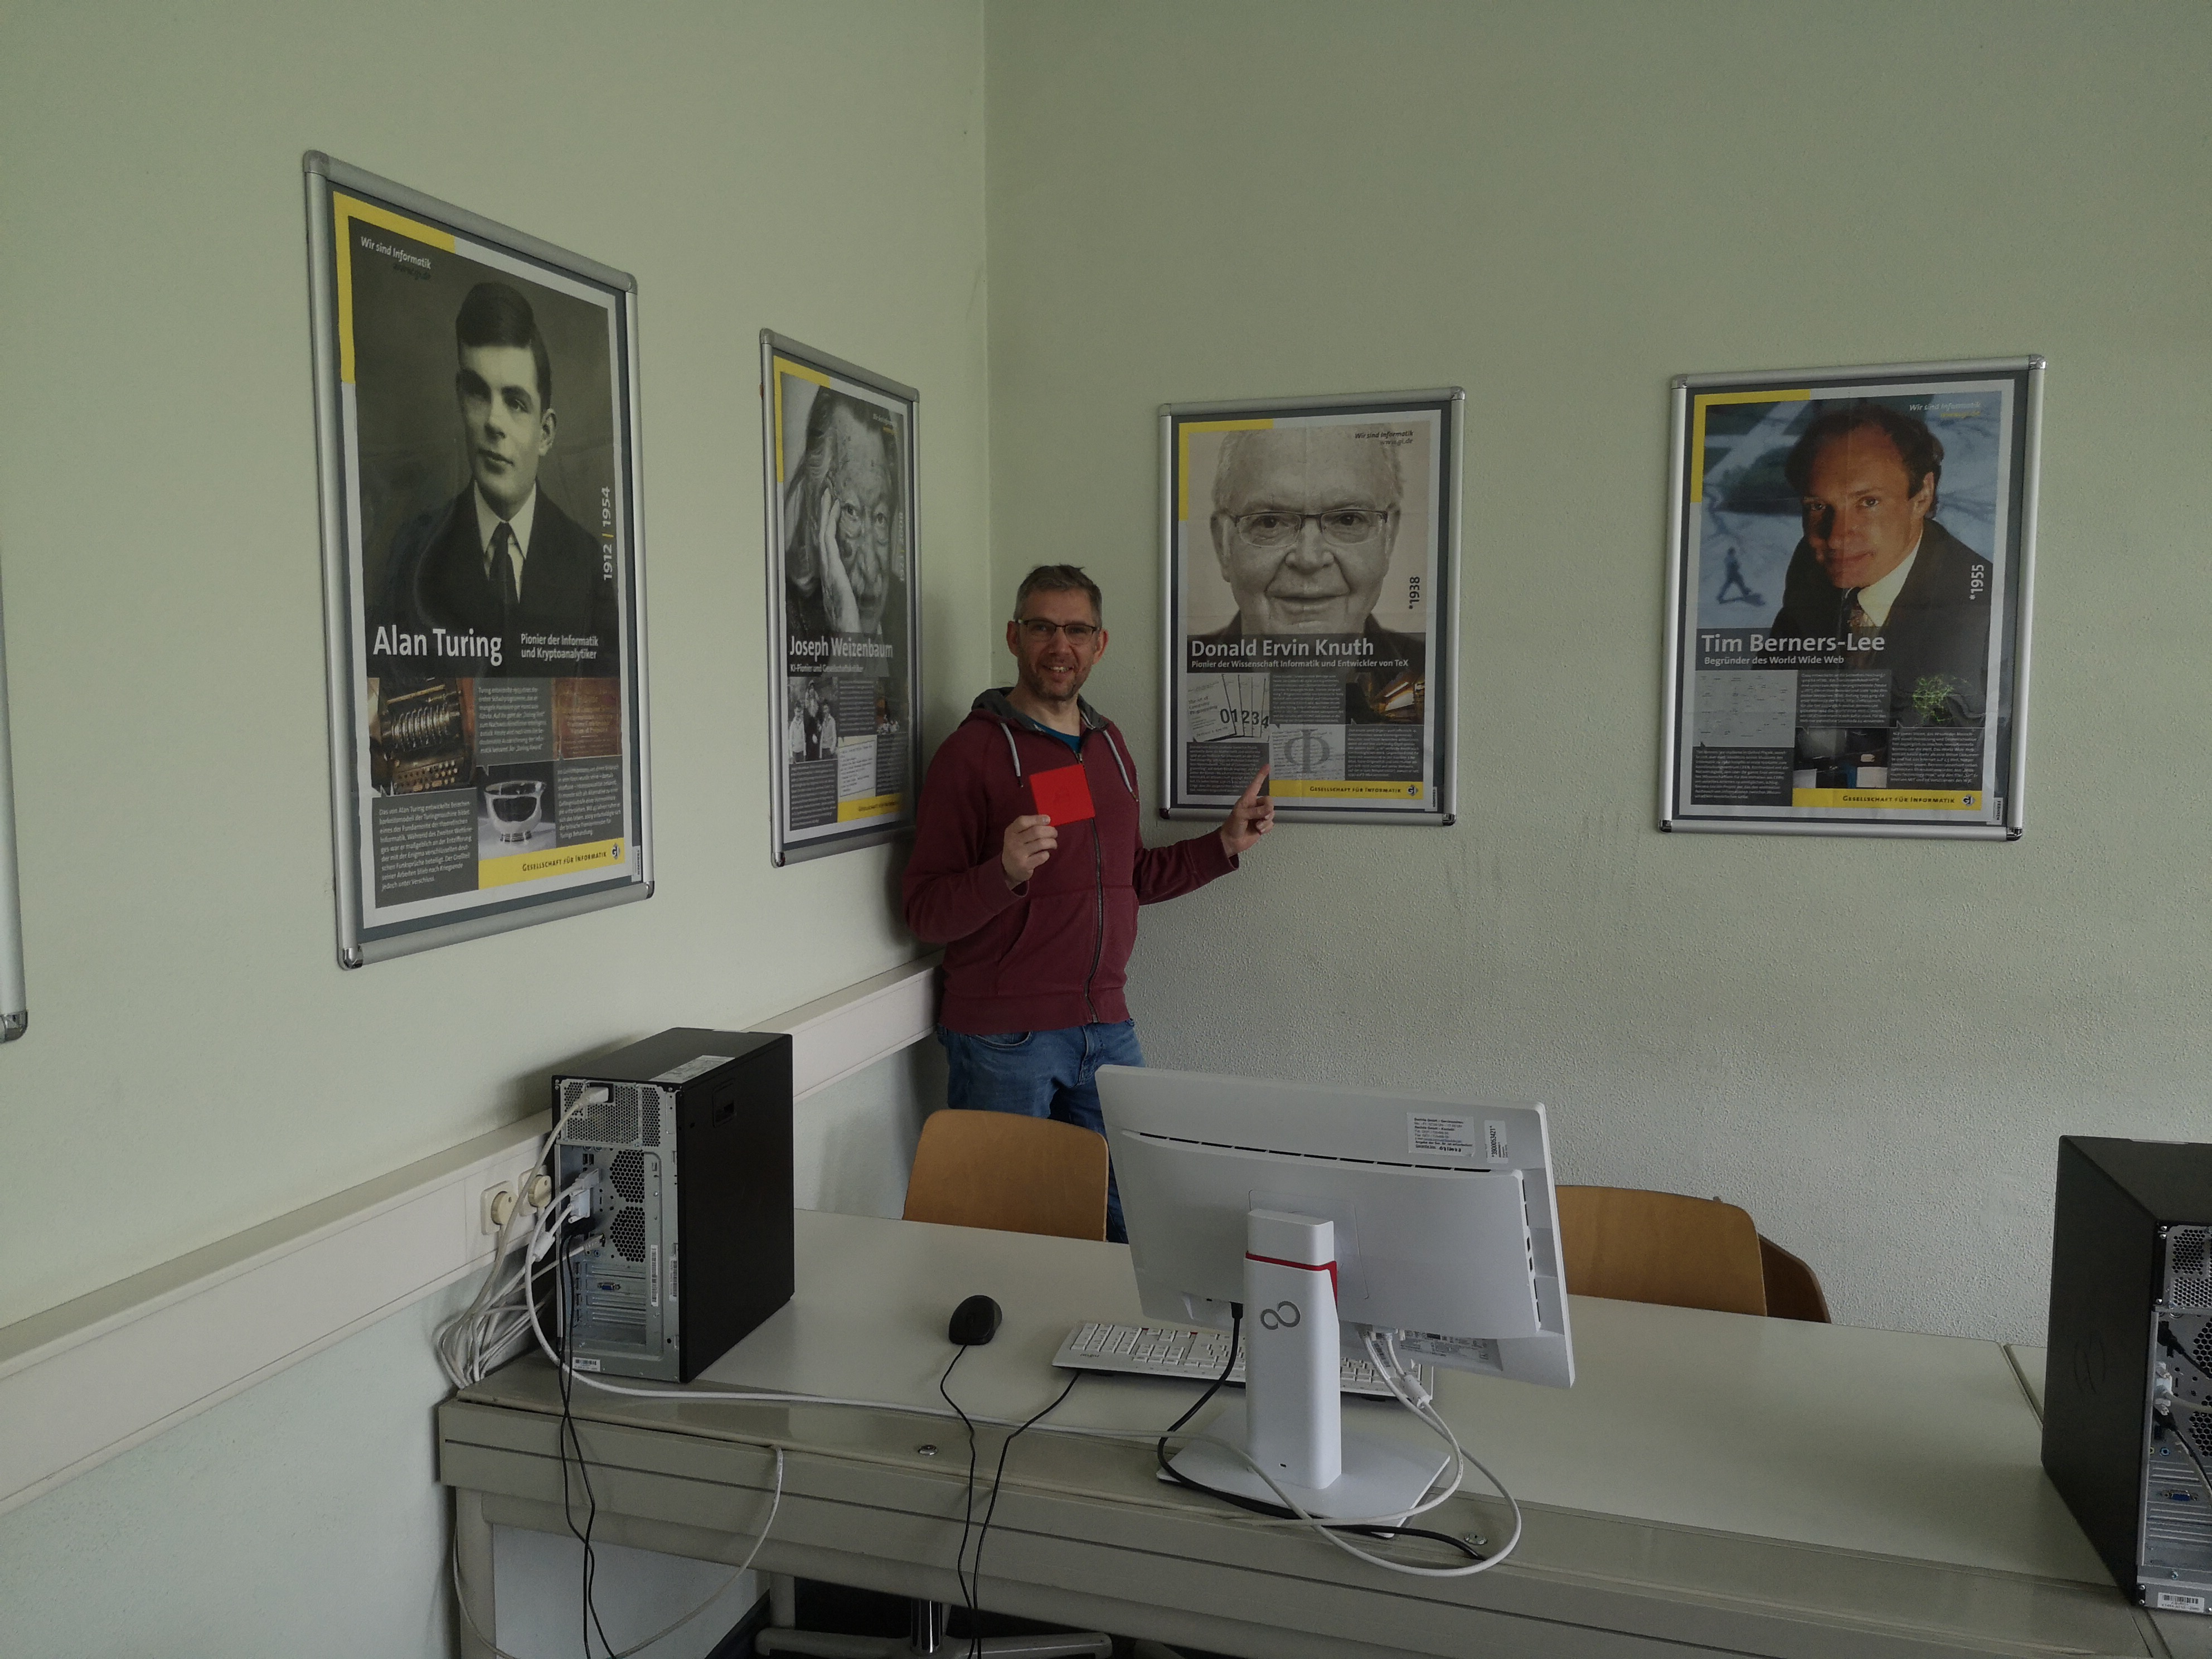
\includegraphics[width=0.7\linewidth]{../poster}


\end{figure}


Thanks for the deal!

I teach CS at a german high school. In our CS lab there is a poster of you (hangs beside Ada Lovelace, Alan Turing, Konrad Zuse and others), where I read, that besides writing TAOCP you are a passionate organ player.

In my home district Köln-Worringen you can find the worldwide first (and probably still unique) "Bierorgel"\footnote{please google: "Bierorgel, Köln Worringen, site:de"}: It's a pipe organ with integrated beer tap! So if you plan to visit Germany give me a call. I surely can arrange you to play on it.

Have fun with the real MIX.




\end{document}
